\section{Schwingungen}

\subsection{Trägheitsmomente}

Brett: $\displaystyle\frac{m}{12} \left(h^2 + b^2\right)$

Stab: $\displaystyle\frac{m}{12} l^2$

Für weitere Trägheitsmomente, siehe \textit{Taschenbuch der Physik} von Horst
Kuchling, Seite 131-132.

\subsection{Pendelschwingungen}

Pendelschwingungen:
\[
	T = 2 \pi \sqrt{\frac{J_S + ma^2}{mga}}	
	\quad \left[ s \right]
\]
Dabei ist $T$ die Schwingungsdauer, $J_S$ das Trägheitsmoment und $a$ der
Abstand vom Schwerpunkt.

Die Schwingungsdauer $T$ entspricht der reziproken Frequenz $1/f$. Die
Kreisfrequenz $\omega$ berechnet sich also wie folgt:
\[
	\omega = 2\pi\frac{1}{T}
\]

\subsection{Wellen}

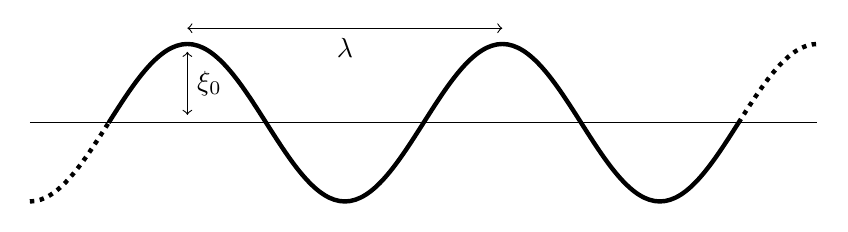
\begin{tikzpicture}

	% Baseline
	\draw (1,0) -- (11,0);

	% Wave
	\draw[x=1cm,y=1cm,dotted,ultra thick] (1,-1) cos (2,0);
	\draw[x=1cm,y=1cm,ultra thick] (2,0)
		sin (3,1) cos (4,0) sin (5,-1) cos (6,0)
		sin (7,1) cos (8,0) sin (9,-1) cos (10,0);
	\draw[x=1cm,y=1cm,dotted,ultra thick] (10,0) sin (11,1);

	% Labels
	\draw[<->] (3,1.2) -- (7,1.2);
	\node[below] at (5,1.2) {$\lambda$};
	\draw[<->] (3,0.1) -- (3,0.9);
	\node[right] at (3,0.5) {$\xi_0$};

\end{tikzpicture}


Frequenz $f$ (manchmal auch als $\nu$ bezeichnet):
\[
	f = \frac{u}{\lambda}
	\quad \left[ \textrm{Hz} \right]
\]
Kreisfrequenz $\omega$:
\[
	\omega = \frac{2 \pi}{T} = 2 \pi f
	\quad \left[ 1/\textrm{s} \right]
\]
Wellenlänge $\lambda$:
\[
	\lambda = \frac{2 \pi}{k} = \frac{u}{f}
	\quad \left[ \textrm{m} \right]
\]
Wellenzahl $k$:
\[
	k = \frac{\omega}{u} = \frac{2 \pi}{\lambda}
	\quad \left[ 1/\textrm{m} \right]
\]
Periode, Schwingungsdauer $T$:
\[
	T = \frac{2 \pi}{\omega}
	\quad \left[ \textrm{s} \right]
\]
Phase $\varphi$:
\[
	\varphi = \omega t - k x
\]
Phasengeschwindigkeit, Wellengeschwindigkeit $u$:
\[
	u = \frac{\omega}{k} = \lambda f
	\quad \left[ \textrm{m} / \textrm{s} \right]
\]
Auslenkung $\xi$ am Ort $x$ zum Zeitpunkt $t$:
\[
	\xi = \xi_0 \sin (\omega t - k x - \varphi_0)
	\quad \left[ \textrm{m} \right]
\]

\subsubsection{Wellenarten}

Wellen, bei denen die Teilchen senkrecht zur Ausbreitungsrichtung der Welle
schwingen, heissen \textbf{Querwellen} / \textbf{Transversalwellen}. In ihnen
wechseln \textbf{Wellenberge} und \textbf{Wellentäler}.

\begin{tikzpicture}
	\draw[->] (0,0) -- (4,0);
	\draw[<->,thick,color=red,<->] (2,.3) -- (2,-.3);
	\node at (2,0) [draw,shape=circle,scale=0.3,color=red,fill=red] {};
\end{tikzpicture}

Sind Schwingungs- und Ausbreitungsrichtung gleich, dann heissen die Wellen
\textbf{Längswellen} / \textbf{Longitudinalwellen}. In ihnen wechseln
\textbf{Verdichtungen} und \textbf{Verdünnungen}.

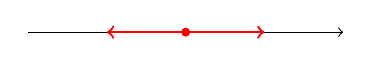
\begin{tikzpicture}
	\draw[->] (0,0) -- (4,0);
	\draw[thick,color=red,<->] (1,0) -- (3,0);
	\node at (2,0) [draw,shape=circle,scale=0.3,color=red,fill=red] {};
\end{tikzpicture}

\subsubsection{Phasensprung}

Wird eine Welle an der Grenze Medium 1 -- Medium 2 ganz oder teilweise
reflektiert, so tritt ein Phasensprung von $\pi$ auf, wenn Medium 2 dichter ist,
d.h. die kleinere Phasengeschwindigkeit $u$ besitzt.

Ein Phasensprung von $\pi$ bedeutet, dass ein ankommender Wellenberg nach der
Reflexion als Wellental zurückläuft (und umgekehrt).

TODO Eigenschwingungen: Grundschwingungen und Oberschwingungen

\subsubsection{Akkustischer Dopplereffekt}

Bewegte Quelle, ruhender Beobachter, kein Winkel:
\[
	f' = \frac{1}{1 \mp \frac{v_Q}{u}} f
\]
Ruhende Quelle, bewegter Beobachter, kein Winkel:
\[
	f' = (1 \pm \frac{v_B}{u}) f
\]
Allgemeine Gleichung mit Winkel $\vartheta$:
\[
	f_B = \frac{u + v_B \cos \vartheta_B}{u - v_Q \cos \vartheta_Q} f_Q
\]
